\section{Dynamic Pipeline Framework in Haskell}\label{dp-hs}
This section presents the design and the main features of the implementation of a general \acrlong{dpf} (\acrshort{hs}).  To be concrete, we present the approach that we follow for designing \acrshort{dpfh}, the system architecture and the  most relevant implementation details.

\subsection{Framework Design}
A suitable framework should provide users with the proper level of abstraction that hides underlying details and allows developers to focus on the problem to be solved. 
%
\iffalse
There are several design approaches to implement a framework: \begin{inparaenum}[i\upshape)]
  \item  \emph{Configuration Based} where users only focus on completing a specific configuration either on a file or a database or both. This configuration is then provided to the runtime system of the framework in order to it executes a customized  program. An example of this could be WordPress\footnote{\url{https://wordpress.com/}}, 
  \item  \emph{Convention over Configuration (CoC)} where users write code and definition following certain patterns in naming or source code location. Using the source code and content-specific information, the framework interprets the execution flow that needs to be executed. This technique has been deeply explored in the last $10$ years. One of the first framework introducing this design paradigm was Ruby on Rails\footnote{\url{https://rubyonrails.org/}}. Other examples are Spring Boot\footnote{\url{https://spring.io/projects/spring-boot}} and Cake PHP\footnote{\url{https://cakephp.org/}},
  \item \emph{Application Programming Interface (API)} where the framework or library provides functions or interfaces. Users need to compose these functions to achieve the desired results. This has been a traditional design approach for building  libraries or frameworks, and finally
  \item \emph{\acrfull{dsl}}~\cite{Fowler10} where the framework or library provides a domain-oriented language. Solutions are written in terms of this \acrshort{dsl} language. An example of this type of design is Hibernate Query Language\footnote{\url{https://docs.jboss.org/hibernate/orm/3.3/reference/en/html/queryhql.html}}
   \end{inparaenum}.
\fi
%
We follow a \acrfull{dsl} approach~\cite{Fowler10} to develop the Dynamic Pipeline Framework in Haskell; it  provides users with a language to write their solutions. There exists two types of \acrlong{dsl}s \cite{dsl}: External \acrfull{dsl} and \acrfull{edsl} \cite{dsel}. The external Domain-Specific Languages (\acrshort{dsl})  are completely new languages requiring the de\-ve\-lop\-ment of an interpreter. On the contrary, the Embedded Domain Specific Languages (\acrshort{edsl}) are languages syntactically embedded in a host language.
Accordingly, actually users write their codes in the host language restricted to the \acrshort{edsl} abstractions. In particular, \acrshort{dpfh} follows an \acrshort{edsl} approach where Haskell is the host language. This approach allows for to take  advantage of the strong type \acrshort{hs}  system to providing correctness at type-level~\cite{curryhoward}. In next definition the Dynamic Pipeline Domain Specific Language (DP-\acrshort{edsl}) is  formally defined.

\begin{definition}\label{def:cfg:dsl}
Syntactical constructions of the Dynamic Pipeline Domain Specific Language (DP-\acrshort{edsl}) are generated by  the grammar $(N, \Sigma, DP, P)$ where
\begin{equation*}\label{grammar:eq}
    %\boxed{
      \begin{aligned}
    N &= \{DP,S_r,S_k,G,F_b,CH,CH_s\},\\
    \Sigma &= \{\text{\mintinline{haskell}{Source}},\text{\mintinline{haskell}{Generator}},\text{\mintinline{haskell}{Sink}},\text{\mintinline{haskell}{FeedbackChannel}},\text{\mintinline{haskell}{Type}},\text{\mintinline{haskell}{Eof}},\text{\mintinline{haskell}{:=>}},\text{\mintinline{haskell}{:<+>}}\},
    \end{aligned}
  %  }
\end{equation*}
\begin{equation*}
  %\boxed{
    \begin{aligned}
  P = \{\\
  DP  &\rightarrow S_r\ \text{\mintinline{haskell}{:=>}}\ G\ \text{\mintinline{haskell}{:=>}}\ S_k\ |\ S_r\ \text{\mintinline{haskell}{:=>}}\ G\ \text{\mintinline{haskell}{:=>}}\ F_b\ \text{\mintinline{haskell}{:=>}}\ S_k,\\
  S_r &\rightarrow \text{\mintinline{haskell}{Source}}\ CH_s,\\
  G   &\rightarrow \text{\mintinline{haskell}{Generator}}\ CH_s,\\
  S_k &\rightarrow \text{\mintinline{haskell}{Sink}},\\
  F_b &\rightarrow \text{\mintinline{haskell}{FeedbackChannel}} CH,\\
  CH_s &\rightarrow \text{\mintinline{haskell}{Channel}}\ CH,\\
  CH &\rightarrow \text{\mintinline{haskell}{Type :<+>}}\ CH\ |\ \text{\mintinline{haskell}{Eof}}\}
\end{aligned}
\end{equation*}
\end{definition}

The configuration of the initial structure of the DP is stated in terms of their connections through channels and the specification of the types of data these channels carry. This configuration is encoded using the DP-\acrshort{edsl}  language. The symbols \text{\mintinline{haskell}{:=>}} and \text{\mintinline{haskell}{:<+>}} allow to separate the encoding of the pipeline stages ($\iwcc$, $\gwcc$, $\owcc$) from the encoding of channel composition in the same stages, respectively.

%
\begin{example}
Consider the problem of defining a DP for removing duplicate elements from a string. The stages are connected by a single channel carrying data of type \texttt{\mintinline{haskell}{Int}}.

\begin{listing}[H]
  \begin{minted}[fontsize=\fontsize{10}{11}\selectfont,numbers=left,breaklines,frame=lines,framerule=2pt,framesep=2mm,baselinestretch=1.2,highlightlines={}]{haskell}

type DPExample = Source (Channel (Int :<+> Eof)) 
              :=> Generator (Channel (Int :<+> Eof)) 
              :=> Sink
   
  \end{minted}
  \caption[{[\mintinline{shell}{Repeated.hs} Example of \acrshort{dp} encoded in $G_{dsl}$}]{Encoding in DP-EDSL of a DP for removing duplicate elements in a stream. Note that the DP is defined at type level of the host language (\acrshort{hs}).}
  \label{src:dpfh:3}
\end{listing}
\end{example}

\paragraph{\textbf{System Architecture}}  The framework has the three components (\autoref{fig:dpfh:1}): EDSL, IDL and RS.\\
%

\begin{figure}[!ht]
  \centering
   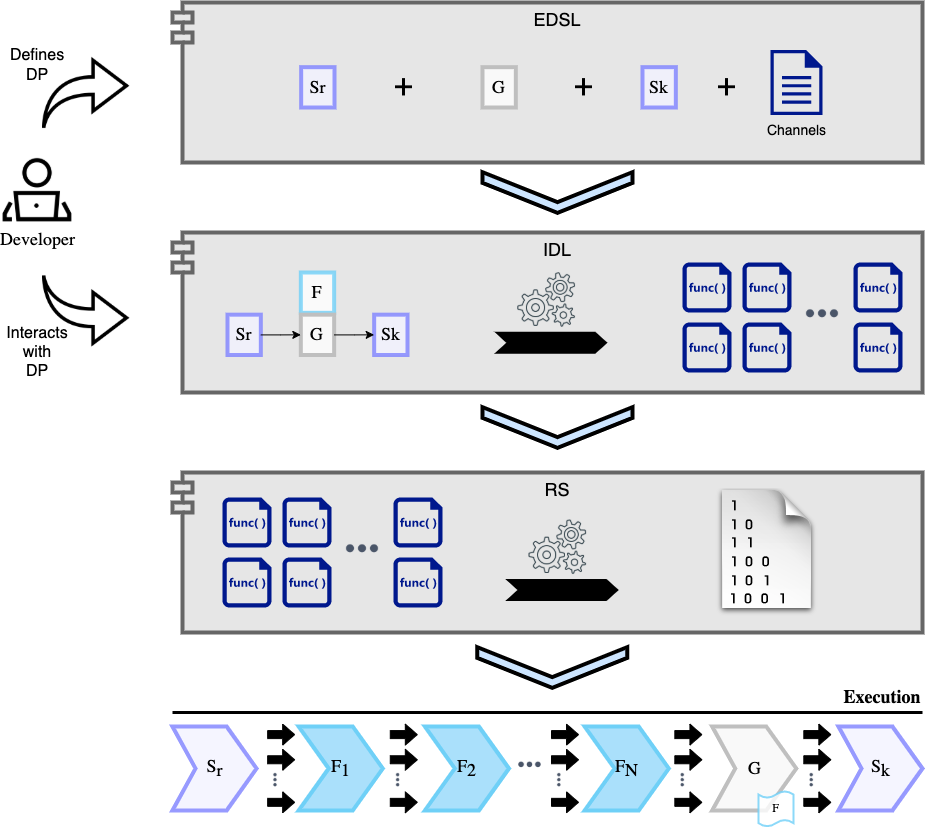
\includegraphics[width=1\textwidth, height=0.6\textheight]{dpf_haskell_v4.png}
    \caption[{[\acrshort{dpfh}] System Architecture of the \acrshort{dpfh}}]{Architecture of the \acrshort{dpfh}. \acrshort{dpfh} is built on three main components: \acrshort{edsl}, \acrshort{idl} and \acrshort{rs}. Users interact with the \acrshort{edsl} and the \acrshort{idl} components. \acrshort{edsl} component allows users to enter the initial stages and  channels specifications. \acrshort{idl} component supports users to define the Haskell functions corresponding to each stage of the DP. Finally \acrshort{rs} execute all that definition plus functions. Execution layer indicates an example of a \acrshort{dp} running after being executed.}
    \label{fig:dpfh:1}
\end{figure}

\paragraph{EDSL Component} This component validates type correctness of the configuration of  the dynamic pipeline to be implemented on top of the  DPF-Haskell.  To do it, it receives from users the DP-\acrshort{edsl} encoding of the initial structure of the DP and a precise specification of the channels connecting the stages of the pipeline. 
%
\paragraph{IDL Component} This component is the Interpreter of the DP specification. According to the structure of the dynamic pipeline provided in the DP-\acrshort{edsl} language, it creates skeletons of the  stages to allow users define each stage in terms of its functions.  Since the Filter stage
is a parameter of the Generator stage, its specification is obtained when Generator is defined. Once users have entered  the Haskell definition of all the stages, the completely defined DP is passed to the Runtime System Component.
%
\paragraph{RS component} This is the Run System component. It receives a Haskell dynamic pipeline definition, compiles it and launch its execution. 
%
\subsection{Implementation}
This section presents 
implementation details of each system component: \acrshort{edsl}, \acrshort{idl} and \acrshort{rs}. 

\begin{listing}[H]
  \begin{minted}[fontsize=\fontsize{10}{11}\selectfont,numbers=left,breaklines,frame=lines,framerule=2pt,framesep=2mm,baselinestretch=1.2,highlightlines={3,4}]{haskell}

data Source (a :: Type)
data Generator (a :: Type)
data Sink
data Eof
data Channel (a :: Type)
data FeedbackChannel (a :: Type)

  \end{minted}
  \caption[{[\mintinline{shell}{Flow.hs}] $\Sigma$ enconding of $G_{dsl}$}]{This code is showing most of the data types that represent the same terminal symbols $\Sigma$ in $G_{dsl}$. These types indexed by another kind \mintinline{haskell}{Type}, allows us to store information at type-level needed for interpret the DP-\acrshort{edsl}}
  \label{src:dpfh:1}
\end{listing}
  

\begin{listing}[H]
  \begin{minted}[fontsize=\fontsize{10}{11}\selectfont,numbers=left,breaklines,frame=lines,framerule=2pt,framesep=2mm,baselinestretch=1.2,highlightlines={1,5}]{haskell}
    
    data chann1 :<+> chann2 = chann1 :<+> chann2
    deriving (Typeable, Eq, Show, Functor, Traversable, Foldable, Bounded)
    infixr 5 :<+>
    
    data a :=> b = a :=> b
    deriving (Typeable, Eq, Show, Functor, Traversable, Foldable, Bounded)
    infixr 5 :=>
    
  \end{minted}
  \caption[{[\mintinline{shell}{Flow.hs}] $\Sigma$ enconding of $G_{dsl}$ - Especial non-terminals}]{Special terminal symbols $\{\text{\mintinline{haskell}{:<+>}}, \text{\mintinline{haskell}{:=>}}\} \subset \Sigma$. These terminal symbols allow us to index two types, in order to combine several of them and build a chain of stages (using \mintinline{haskell}{:=>}) and a set of channels (using \mintinline{haskell}{:<+>}).}
  \label{src:dpfh:2}
\end{listing}

\subsubsection{EDSL Validation}\label{sub:sec:dsl-val}
First, let us pay attention to the embedding of the DP-\acrshort{edsl} into \acrshort{hs}. For this purpose we use an Index type \cite{type-index} that allows for keeping track –at type-level– of the extra information required by the DP definition, i.e., channels and data types carried by the channels. In \autoref{src:dpfh:1}, an \emph{Index type} for each element of $\Sigma$ an \emph{Index type} is defined to encoded them in \acrshort{hs} types. Note that  \mintinline{haskell}{Sink} and  \mintinline{haskell}{Eof} are not indexed. This is because these symbols do not carry extra type-level information. In the case of \mintinline{haskell}{Sink}, since it is the last stage that does not connect further with any other stage, we do not need to indicate any channel information.  \mintinline{haskell}{Eof} is just a terminal type to disambiguate the \mintinline{haskell}{Channel (a :: Type)} of the tree branch. \mintinline{haskell}{Channel} can carry any type of data because it is polymorphic to support different number of channels and data types. 
In \autoref{src:dpfh:2}, the type definition shows how \mintinline{haskell}{:=>} and \mintinline{haskell}{:<+>} can combine two types.  Writing \mintinline{haskell}{:=>} and \mintinline{haskell}{:<+>} as types is to have a syntactic sugar type combinator in the DP-\acrshort{edsl}. 

The DP-\acrshort{edsl} code (with the syntactical constructions from Definition \ref{def:cfg:dsl}) provided by users must be compiled. Fortunately, \acrshort{hs} provides several type-level techniques~\cite{type-haskell} that allow for verifying properties of programs before running them. This prevents users to introduce bugs and hence to reduce the occurrence of  errors. This verification done by the compiler establish a Curry-Howard Isomorphism~\cite{curryhoward}, i.e., \emph{Propositions as Types - Programs as Proof}. It is important to remark that \acrshort{hs} is not a theorem prover system like Coq\footnote{\url{https://coq.inria.fr/}}, but some verifications, as we present in this work, can be done by the \acrshort{ghc} (Glasgow Haskell Compiler) to ensure correctness on programs.
Although, \acrshort{hs} provides tools to build advanced type-level verification, all these techniques require the use  of \emph{Haskell Language Extensions}.


\begin{listing}[b!]
 \scriptsize{
  \begin{minted}[fontsize=\fontsize{10}{11}\selectfont,numbers=left,breaklines,frame=lines,framerule=2pt,framesep=2mm,baselinestretch=1.2,highlightlines={6,18}]{haskell}

type family And (a :: Bool) (b :: Bool) :: Bool where
    And 'True 'True = 'True
    And a b         = 'False
  

type family IsDP (dpDefinition :: k) :: Bool where
    IsDP (Source (Channel inToGen) :=> Generator (Channel genToOut) :=> Sink)
        = And (IsDP (Source (Channel inToGen))) (IsDP (Generator (Channel genToOut)))
    IsDP ( Source (Channel inToGen) :=> Generator (Channel genToOut) :=> FeedbackChannel toSource :=> Sink)
        = And (IsDP (Source (Channel inToGen))) (IsDP (Generator (Channel genToOut)))
    IsDP (Source (Channel (a :<+> more)))     
        = IsDP (Source (Channel more))
    IsDP (Source (Channel Eof))               = 'True
    IsDP (Generator (Channel (a :<+> more)))  = IsDP (Generator (Channel more))
    IsDP (Generator (Channel a))              = 'True
    IsDP x                                    = 'False
     
type family ValidDP (a :: Bool) :: Constraint where
  ValidDP 'True = ()
  ValidDP 'False = TypeError
                    ( 'Text "Invalid Semantic for Building DP Program"
                      ':$$: 'Text "Language Grammar:"
                      ':$$: 'Text "DP       -> Source CHANS :=> Generator CHANS :=> Sink"
                      ':$$: 'Text "DP       -> Source CHANS :=> Generator CHANS :=> FEEDBACK :=> Sink"
                      ':$$: 'Text "CHANS    -> Channel CH"
                      ':$$: 'Text "FEEDBACK -> FeedbackChannel CH"
                      ':$$: 'Text "CH       -> Type :<+> CH | Eof"
                      ':$$: 'Text "Example: 'Source (Channel (Int :<+> Int)) :=> Generator (Channel (Int :<+> Int)) :=> Sink'"
                    )
  \end{minted}
  }
  \caption[{[\mintinline{shell}{Stage.hs}] Validating DP-\acrshort{edsl} code - FCF}]{Type Families \mintinline{haskell}{And}, \mintinline{haskell}{IsDP} and \mintinline{haskell}{ValidDP} that allow to perform a type-level validation over a DP-\acrshort{edsl} \acrshort{cfg} definition.}
  \label{src:dpfh:4}
\end{listing}

The implementation of the validation is done using \emph{Associated Type Families}~\cite{associated-types}. 
In \autoref{src:dpfh:4}, there are three Type families that help to validate the DP-\acrshort{edsl} code. 
\mintinline{haskell}{IsDP} associated type family is checking the production rules $P$ of the grammar defined in \dref{grammar:eq}, returning a promoted data type~\cite{promoted-types} (not a boolean value) \mintinline{haskell}{'True} in case the production rule matches all the generated language, or \mintinline{haskell}{'False} otherwise. 
\mintinline{haskell}{ValidDP} is taking the result of \mintinline{haskell}{IsDP} type application, associating \mintinline{haskell}{'True} promoted boolean type to empty \mintinline{haskell}{()} constraint. An empty constraint is an indication of no restriction, i.e., if \mintinline{haskell}{ValidDP} is used as a constraint. It is fully applied to \mintinline{haskell}{()} and gives the compiler the evidence that there is no error at type-level.
\mintinline{haskell}{ValidDP} is also associating \mintinline{haskell}{'False} with a custom \mintinline{haskell}{TypeError}; it will appear at compilation time if the DP-\acrshort{edsl} definition fully applies to that -- a type checked error --.

\iffalse
In \autoref{src:dpfh:4}, there are three Type families that help to validate the DP-\acrshort{edsl} code. 
\mintinline{haskell}{IsDP} associated type family is checking the production rules $P$ of the grammar defined in \dref{grammar:eq}, returning a promoted data type~\cite{promoted-types} (not a boolean value) \mintinline{haskell}{'True} in case the production rule matches all the generated language, or \mintinline{haskell}{'False} otherwise. 
\mintinline{haskell}{ValidDP} is taking the result of \mintinline{haskell}{IsDP} type application, associating \mintinline{haskell}{'True} promoted boolean type to empty \mintinline{haskell}{()} constraint. An empty constraint is an indication of no restriction, i.e., if \mintinline{haskell}{ValidDP} is used as a constraint. It is fully applied to \mintinline{haskell}{()} and gives the compiler the evidence that there is no error at type-level.
\mintinline{haskell}{ValidDP} is also associating \mintinline{haskell}{'False} with a custom \mintinline{haskell}{TypeError}; it will appear at compilation time if the DP-\acrshort{edsl} definition fully applies to that -- a type checked error --.
\fi

\begin{listing}[H]
  \begin{minted}[fontsize=\fontsize{10}{11}\selectfont,numbers=left,breaklines,frame=lines,framerule=2pt,framesep=2mm,baselinestretch=1.2,highlightlines={2}]{haskell}

mkDP :: forall dpDefinition filterState filterParam st.
    ( ValidDP (IsDP dpDefinition)
    , DPConstraint dpDefinition filterState st filterParam)
 => Stage (WithSource dpDefinition (DP st)) 
 -> GeneratorStage dpDefinition filterState filterParam st  
 -> Stage (WithSink dpDefinition (DP st))  
 -> DP st ()
mkDP = ...

someFunc = mkDP @DPExample ...

  \end{minted}
  \caption[{[\mintinline{shell}{Stage.hs}] Using validation of \acrshort{dp} encoded in $G_{dsl}$}]{Definition of \mintinline{haskell}{mkDP} function of the Framework which uses type-level validation of DP-\acrshort{edsl} code \mintinline{haskell}{ValidDP (IsValid Type)}. Last line of the code is showing that using that function will compile-time check the definition of \mintinline{haskell}{DPExample} type (\autoref{src:dpfh:3})}
  \label{src:dpfh:5}
\end{listing}

\subsubsection{\texorpdfstring{\acrfull{idl}}{Lg}}
\acrshort{idl} component takes the dynamic pipeline specification made on with DP-\acrshort{edsl} component to interpret and generate the function definitions that needs to be implemented for solving a specific problem. In \autoref{sec:dp}, we describe what should be provided in a \acrshort{dp} algorithm. % $\iwcc$, $\gwcc$, $\owcc$, and the $\fwcc$ with the non-empty set of Actors.
The \acrshort{idl} generates the function definitions with an empty implementation to be entered by users, ensuring that those functions will give "Proof" -- in terms of Curry-Howard Correspondence~\cite{curryhoward} --  of the "Propositions" defined on the DP-\acrshort{edsl}.
\acrshort{idl} utilizes techniques similar to the ones used in \autoref{sub:sec:dsl-val}. First, \emph{Type-level Defunctionalization}~\cite{defunctionalization, fun-type-function-haskell} is used to let the compiler generates the signatures of the required functions. 
Second, \emph{Term-level Defunctionalization} interprets those functions.
Lastly, \emph{Indexed Types}~\cite{type-index} and \emph{Heterogeneous List}~\cite{hlist} keep track of the dynamic number and polymorphic types of the functions parameters. 

\begin{listing}[H]
  \begin{minted}[fontsize=\fontsize{10}{11}\selectfont,numbers=left,breaklines,frame=lines,framerule=2pt,framesep=2mm,baselinestretch=1.2,highlightlines={2,6,10}]{haskell}
withSource :: forall (dpDefinition :: Type) st. WithSource dpDefinition (DP st) 
            -> Stage (WithSource dpDefinition (DP st))
withSource = mkStage' @(WithSource dpDefinition (DP st))

withGenerator :: forall (dpDefinition :: Type) (filter :: Type) st. WithGenerator dpDefinition filter (DP st) 
              -> Stage (WithGenerator dpDefinition filter (DP st))
withGenerator = mkStage' @(WithGenerator dpDefinition filter (DP st))

withSink :: forall (dpDefinition :: Type) st. WithSink dpDefinition (DP st) 
           -> Stage (WithSink dpDefinition (DP st))
withSink = mkStage' @(WithSink dpDefinition (DP st))
  \end{minted}
  \caption[{[\mintinline{shell}{Stage.hs}] Using with Interpreters of \acrshort{dp} encoded in $G_{dsl}$}]{This code is showing the different interpreters combinators to support users to generate the functions of the stages of the dynamic pipeline}
  \label{src:dpfh:6}
\end{listing}

In \autoref{src:dpfh:6}, we can appreciate the different combinators of the \acrshort{idl} that help to interpret the DP-\acrshort{edsl} and generates the function definitions.
\mintinline[breaklines]{haskell}{Stage} data type will be cover in \autoref{src:dpfh:8}, but it is a wrapper type of a pipeline stage -- minimal unit of execution --, containing the function to be executed -- here is the use \emph{Term-level Defunctionalization} --.
\mintinline[breaklines]{haskell}{withSource}, \mintinline[breaklines]{haskell}{withGenerator}, and \mintinline[breaklines]{haskell}{withSink} are aliases of the function \mintinline[breaklines]{haskell}{mkStage'} which is the combinator that is applying the \emph{Associated Type} related to that stage. For example \mintinline[breaklines]{haskell}{withSource}, is equivalent to \mintinline[breaklines]{haskell}{mkStage' @(WithSource dpDefinition (DP st))}.
For each \emph{Associated Type Family} definition, there is an equivalent term-level definition: \mintinline[breaklines]{haskell}{WithSource} type with \mintinline[breaklines]{haskell}{withSource} term , \mintinline[breaklines]{haskell}{WithGenerator} type with \mintinline[breaklines]{haskell}{withGenerator} term, and \mintinline[breaklines]{haskell}{WithSink} type with \mintinline[breaklines]{haskell}{withSink} term -- notice the capital case letter "W" indicating the type and not the term --.

\begin{listing}[b!]
 \scriptsize{
  \begin{minted}[fontsize=\fontsize{10}{11}\selectfont,numbers=left,breaklines,frame=lines,framerule=2pt,framesep=2mm,baselinestretch=1.2,highlightlines={7,11}]{haskell}
type family WithSource (dpDefinition :: Type) (monadicAction :: Type -> Type) :: Type where
  WithSource (Source (Channel inToGen) :=> Generator (Channel genToOut) :=> Sink) monadicAction
      = WithSource (ChanIn inToGen) monadicAction
  WithSource (Source (Channel inToGen) :=> Generator (Channel genToOut) :=> FeedbackChannel toSource :=> Sink) monadicAction 
      = WithSource (ChanOutIn toSource inToGen) monadicAction
  WithSource (ChanIn (dpDefinition :<+> more)) monadicAction         
      = WriteChannel dpDefinition -> WithSource (ChanIn more) monadicAction
  WithSource (ChanIn Eof) monadicAction                              
      = monadicAction ()
  WithSource (ChanOutIn (dpDefinition :<+> more) ins) monadicAction  
      = ReadChannel dpDefinition -> WithSource (ChanOutIn more ins) monadicAction
  WithSource (ChanOutIn Eof ins) monadicAction                       
      = WithSource (ChanIn ins) monadicAction
  WithSource dpDefinition _                                          
      = TypeError
          ( 'Text "Invalid Semantic for Source Stage"
            ':$$: 'Text "in the DP Definition '"
            ':<>: 'ShowType dpDefinition
            ':<>: 'Text "'"
            ':$$: 'Text "Language Grammar:"
            ':$$: 'Text "DP       -> Source CHANS :=> Generator CHANS :=> Sink"
            ':$$: 'Text "DP       -> Source CHANS :=> Generator CHANS :=> FEEDBACK :=> Sink"
            ':$$: 'Text "CHANS    -> Channel CH"
            ':$$: 'Text "FEEDBACK -> FeedbackChannel CH"
            ':$$: 'Text "CH       -> Type :<+> CH | Eof"
            ':$$: 'Text "Example: 'Source (Channel (Int :<+> Int)) :=> Generator (Channel (Int :<+> Int)) :=> Sink'"
          )
  \end{minted}
  }
  \caption[{[\mintinline{shell}{Stage.hs}] WithSource Associate Type Details}]{An example of the Associated Type Family \mintinline{haskell}{WithSource} that allows to implement \emph{Type-level Defunctionalization} technique that will be the Type-level verification of the term \mintinline{haskell}{withSource}}
  \label{src:dpfh:7}
\end{listing}

In \autoref{src:dpfh:7}, in the highlighted lines, it can be seen how \emph{Type-level Defunctionalization} is being expanded in a signature function definition with the form \mintinline[breaklines]{haskell}{WriteChannel a -> ReadChannel b -> ... -> monadicAction ()} depending on \acrshort{dp} language definition. 

\begin{listing}[h!]
 \scriptsize{
  \begin{minted}[fontsize=\fontsize{10}{11}\selectfont,numbers=left,breaklines,frame=lines,framerule=2pt,framesep=2mm,baselinestretch=1.2,highlightlines={12,16}]{haskell}

data Stage a where
  Stage :: Proxy a -> a -> Stage a

mkStage' :: forall a. a -> Stage a
mkStage' = Stage (Proxy @a)
    
  \end{minted}
  }
  \caption[{[\mintinline{shell}{Stage.hs}] Stage Data Type}]{\mintinline{haskell}{Stage} data type for implementing \emph{Term-level Defunctionalization} providing evidence to the Type-Level Associated types}
  \label{src:dpfh:8}
\end{listing}

In \autoref{src:dpfh:8}, \mintinline{haskell}{Stage} data type uses a \mintinline{haskell}{Proxy} type. 
This \mintinline{haskell}{Proxy} type allows \mintinline{haskell}{Stage} to index the type definition generated by \mintinline{haskell}{a}.
For example, in \autoref{src:dpfh:6}, when \mintinline{haskell}{withSource} interpreter is applied to \mintinline{haskell}{WithSource dpDefinition},  
the compiler is provided with \mintinline{haskell}{dpDefinition} \acrshort{dsl} type, expanding the function signature belonging to that \acrshort{dp} definition inside the \mintinline{haskell}{Stage}.

\paragraph{Generator and Filter}
According to \acrshort{dp} definition in \autoref{sec:dp}, the Generator ($\gwcc$) stage has a Filter ($\fwcc$) template as parameter. In order to know how to dynamically interpose a new $\fwcc$ during the runtime execution of the program let us first study $\fwcc$ Data Type in the context of the framework.

\begin{listing}[h!]
 \scriptsize{
  \begin{minted}[fontsize=\fontsize{10}{11}\selectfont,numbers=left,breaklines,frame=lines,framerule=2pt,framesep=2mm,baselinestretch=1.2,highlightlines={2,5}]{haskell}

newtype Actor dpDefinition filterState filterParam monadicAction =
    Actor {  unActor :: MonadState filterState monadicAction => Stage (WithFilter dpDefinition filterParam monadicAction) }

newtype Filter dpDefinition filterState filterParam st =
    Filter { unFilter :: NonEmpty (Actor dpDefinition filterState filterParam (StateT filterState (DP st))) }
    deriving Generic
    
  \end{minted}
  }
  \caption[{[\mintinline{shell}{Stage.hs}] Filter / Actor Data Type}]{This code shows the definition of the \mintinline{haskell}{Filter} data type which contains a non-empty set of \mintinline{haskell}{Actor}. In the Context of the \mintinline{haskell}{MonadState} the data type of  \mintinline{haskell}{Actor} is  \mintinline{haskell}{Stage}. This allows for keeping a local memory in the execution context of the filter.}
  \label{src:dpfh:9}
\end{listing}

In \autoref{src:dpfh:9}, the definition of the \mintinline{haskell}{Filter} data type contains a non-empty set of \mintinline{haskell}{Actor}.
An \mintinline{haskell}{Actor} is the minimal unit of execution of a filter. 
A \mintinline{haskell}{Filter} has a \mintinline{haskell}{NonEmpty Actor} -- Non-empty List -- because a filter is built by a sequence of actors calls. 
Moreover, \mintinline{haskell}{Actor} Stage is defunctionalized with \mintinline{haskell}{WithFilter} \emph{Associated Type Family}. 
\mintinline{haskell}{Filter} runs in an explicit \mintinline{haskell}{StateT} monadic context. This is because the $\fwcc$ instance should have an state, according to \acrshort{dp} definition in \autoref{sec:dp}. 
\mintinline{haskell}{Actor} data type -- see \autoref{src:dpfh:9} --, is constrained by \mintinline{haskell}{MonadState} which is in the same execution context of the whole \mintinline{haskell}{NonEmpty Actor} list of the \mintinline{haskell}{Filter}. 
This means the \mintinline{haskell}{StateT} is executed for each \mintinline{haskell}{Actor} of that filter, sharing the same state between them. 

\begin{listing}[h!]
 \scriptsize{
  \begin{minted}[fontsize=\fontsize{10}{11}\selectfont,numbers=left,breaklines,frame=lines,framerule=2pt,framesep=2mm,baselinestretch=1.2,highlightlines={}]{haskell}

mkFilter :: forall dpDefinition filterState filterParam st. WithFilter dpDefinition filterParam (StateT filterState (DP st)) 
         -> Filter dpDefinition filterState filterParam st
mkFilter = Filter . single

single :: forall dpDefinition filterState filterParam st. WithFilter dpDefinition filterParam (StateT filterState (DP st)) 
       -> NonEmpty (Actor dpDefinition filterState filterParam (StateT filterState (DP st)))
single = one . actor

actor :: forall dpDefinition filterState filterParam st. WithFilter dpDefinition filterParam (StateT filterState (DP st)) 
      -> Actor dpDefinition filterState filterParam (StateT filterState (DP st))
actor = Actor . mkStage' @(WithFilter dpDefinition filterParam (StateT filterState (DP st)))

(|>>>) :: forall dpDefinition filterState filterParam st. Actor dpDefinition filterState filterParam (StateT filterState (DP st)) 
       -> Filter dpDefinition filterState filterParam st 
       -> Filter dpDefinition filterState filterParam st
(|>>>) a f = f & _Wrapped' %~ (a <|)
infixr 5 |>>>

(|>>) :: forall dpDefinition filterState filterParam st. Actor dpDefinition filterState filterParam (StateT filterState (DP st)) 
      -> Actor dpDefinition filterState filterParam (StateT filterState (DP st)) 
      -> Filter dpDefinition filterState filterParam st
(|>>) a1 a2 = Filter (a1 <|one a2)
infixr 5 |>>
  \end{minted}
  }
  \caption[{[\mintinline{shell}{Stage.hs}] Filter / Actor smart constructors and combinators}]{Combinators and small constructor to enable building actors and filter.}
  \label{src:dpfh:10}
\end{listing}

Finally, in \autoref{src:dpfh:10}, some combinators and smart constructors are provided in the framework to enable the construction of \mintinline{haskell}{Filter} and \mintinline{haskell}{Actor}.
\mintinline{haskell}{mkFilter} is a smart constructor for \mintinline{haskell}{Filter} Data Constructor. \mintinline{haskell}{single} wraps one actor inside a \mintinline{haskell}{Filter}.
\mintinline{haskell}{actor} is a smart constructor for \mintinline{haskell}{Actor} Data Constructor. \mintinline{haskell}{(|>>>)} is an appending combinator of an \mintinline{haskell}{Actor} to a \mintinline{haskell}{Filter}. 
\mintinline{haskell}{(|>>>)} also ensures actor execution order, i.e., the latest actor added is the latest to be executed.


\begin{listing}[h!]
 \scriptsize{
  \begin{minted}[fontsize=\fontsize{10}{11}\selectfont,numbers=left,breaklines,frame=lines,framerule=2pt,framesep=2mm,baselinestretch=1.2,highlightlines={}]{haskell}
    data GeneratorStage dpDefinition filterState filterParam st = GeneratorStage
    { _gsGenerator      :: Stage (WithGenerator dpDefinition (Filter dpDefinition filterState filterParam st) (DP st))
    , _gsFilterTemplate :: Filter dpDefinition filterState filterParam st
    }  
  \end{minted}
  }
  \caption[{[\mintinline{shell}{Stage.hs}] Generator}]{\mintinline{haskell}{Generator} Data type which contains the \mintinline{haskell}{Stage} code of the generator itself, and the \mintinline{haskell}{Filter} template that can be spawned by the \mintinline{haskell}{Generator}.}
  \label{src:dpfh:11}
\end{listing}

In \autoref{src:dpfh:11}, $\gwcc$ contains a $\fwcc$ template and its own stage behavior.
\mintinline{haskell}{Generator} data type has a field with the \mintinline{haskell}{Filter} template that could be spawned by the algorithms defined by users according to the data received from its input channels.
\mintinline{haskell}{Generator} has also another field with the behavior of the $\gwcc$ -- a \mintinline{haskell}{Stage} --. 

\subsubsection{\texorpdfstring{\acrfull{rs}}{Lg}}
The \acrshort{rs} can be divided into two parts: the mechanism to generate stages dynamically at runtime  and the execution entry point of the DP.
Regarding execution entry point, all the stages defined above are the pieces needed to build an executable \mintinline{haskell}{DP st a} monad.
This executable monad has an existential type similar to \mintinline{haskell}{ST} monad to not escape out from the context on different stages.
Once the dynamic pipeline starts to execute, the core of the framework dynamically generates stages between $\gwcc$ and previous stages, according to users definitions, i.e., an \emph{anamorphism}~\cite{lenses} that creates $\fwcc$ instances until some condition is met.

\begin{listing}[H]
  \begin{minted}[fontsize=\fontsize{10}{11}\selectfont,numbers=left,breaklines,frame=lines,framerule=2pt,framesep=2mm,baselinestretch=1.2,highlightlines={2,12,14,15,16,17,18}]{haskell}
unfoldF :: forall dpDefinition readElem st filterState filterParam l. SpawnFilterConstraint dpDefinition readElem st filterState filterParam l
        => UnFoldFilter dpDefinition readElem st filterState filterParam l 
        -> DP st (HList l) 
unfoldF = loopSpawn

where
  loopSpawn uf@UnFoldFilter{..} =
    maybe (pure _ufRsChannels) (loopSpawn <=< doOnElem uf) =<< DP (pull _ufReadChannel)

  doOnElem uf@UnFoldFilter{..} elem' = do
    _ufOnElem elem'
    if _ufSpawnIf elem'
     then do
       (reads', writes' :: HList l3) <- getFilterChannels <$> DP (makeChansF @(ChansFilter dpDefinition))
       let hlist = elem' .*. _ufReadChannel .*. (_ufRsChannels `hAppendList` writes')
       void $ runFilter _ufFilter (_ufInitState elem') hlist (_ufReadChannel .*. (_ufRsChannels `hAppendList` writes'))
       return $ uf { _ufReadChannel = hHead reads', _ufRsChannels = hTail reads' }
     else return uf

  \end{minted}
  \caption[{[\mintinline{shell}{Stage.hs}] unfoldF}]{\mintinline{haskell}{unfolF} is the \emph{anamorphism} combinator to spawn new \mintinline{haskell}{Filter} types between the \mintinline{haskell}{Generator} and previous stages.}
  \label{src:dpfh:12}
\end{listing}

In \autoref{src:dpfh:12}, it is presented how is the \emph{anamorphism} mechanim that generates dynamic stages between $\gwcc$ and the previous stages.
This \emph{anamorphism} is implemented with the function \mintinline{haskell}{unfoldF}. This function receives an \mintinline{haskell}{UnFoldFilter} Data type, which contains the recipe for controlling that unfold recursive call. 
In line $12$, \mintinline{haskell}{_ufSpawnIf} field of \mintinline{haskell}{UnFoldFilter}, indicates when to stop the recursion. 
Inside the conditional, in line $14$, new channels are created for the new filter to be spawned. New channels connect the new filter with the previous stages and with \mintinline{haskell}{Generator}. 
After that, in line $16$ \mintinline{haskell}{runFilter} starts the monadic computation, spawning the filter stage with its actors.
Finally, the new list of channels are returned for the next recursive step to allow further channel connections.

\begin{listing}[h!]
 \scriptsize{
  \begin{minted}[fontsize=\fontsize{10}{11}\selectfont,numbers=left,breaklines,frame=lines,framerule=2pt,framesep=2mm,baselinestretch=1.2,highlightlines={}]{haskell}
mkUnfoldFilter :: (readElem -> Bool) 
    -> (readElem -> DP st ()) 
    -> Filter dpDefinition filterState filterParam st 
    -> (readElem -> filterState)
    -> ReadChannel readElem
    -> HList l 
    -> UnFoldFilter dpDefinition readElem st filterState filterParam l


mkUnfoldFilterForAll' :: (readElem -> DP st ())
                      -> Filter dpDefinition filterState filterParam st
                      -> (readElem -> filterState)
                      -> ReadChannel readElem
                      -> HList l
                      -> UnFoldFilter dpDefinition readElem st filterState filterParam l

mkUnfoldFilterForAll :: Filter dpDefinition filterState filterParam st
                      -> (readElem -> filterState)
                      -> ReadChannel readElem
                      -> HList l
                      -> UnFoldFilter dpDefinition readElem st filterState filterParam l
   \end{minted}
   }
  \caption[{[\mintinline{shell}{Stage.hs}] UnfoldFilter combinators}]{Combinators for building \mintinline{haskell}{UnfoldFilter} types indicating the type of the \mintinline{haskell}{unfold} that users want to achieve.}
  \label{src:dpfh:13}
\end{listing}

Several smart constructors are also provided for building \mintinline{haskell}{UnfoldFilter} Data Type.
In \autoref{src:dpfh:13} the first combinator is the default smart constructor.  \begin{inparaenum}[i\upshape)]
  \item First field \mintinline{haskell}{(readElem -> Bool)} indicate if the a new filter should be spawn or not.
  \item The second field \mintinline{haskell}{(readElem -> DP st ())} is a monadic optional computation to do when received a new element, for example logging.
  \item Third field \mintinline{haskell}{Filter} data type to be spawned.
  \item Fourth field \mintinline{haskell}{(readElem -> filterState)} is initialization of the \mintinline{haskell}{Filter} State.
  \item Fifth field \mintinline{haskell}{(ReadChannel readElem)} that feeds the filter instance.
  \item Last field is the \emph{Heterogeneous List} with the rest of the channels to connect with other stages.
\end{inparaenum}
The combinator \mintinline{haskell}{mkUnfoldFilterForAll} is a smart constructor of \mintinline{haskell}{UnfoldFilter} that allows to spawn a new filter for each element received in the $\gwcc$.

\subsection{Libraries and Tools}
%\paragraph{Parallelization} 
One of the most important task of the implementation is the selection of concurrency libraries to support an intensive parallelization workload. Parallelization techniques and tools have been intensively studied and implemented in \acrshort{hs} \cite{monadpar}. 
Indeed, it is well known that green threads and sparks allow spawning thousands to millions of parallel computations. 
These parallel computations do not penalize performance when compare with \acrfull{os} level threading \cite{parallelbook}. 
A straightforward assumption to achieve, here, is to use \texttt{monad-par} library\footnote{\url{https://hackage.haskell.org/package/monad-par}}. 
But, in this first version of the \acrshort{dpfh} we do not use  sparks \cite{sparks1, sparks} but spawning green threads only. We will consider the use of sparks for future versions.
Another choice is to use:
\mintinline{haskell}{forkIO :: IO () -> IO ThreadId} from \texttt{base} library\footnote{\url{https://hackage.haskell.org/package/base-4.15.0.0/docs/Control-Concurrent.html}}. 
However, that would imply handling all the threads lifecycles and errors programmatically without any abstraction to facilitate that complex task. 
Therefore, we choose \texttt{async} library\footnote{\url{https://hackage.haskell.org/package/async}} which enables to spawn asynchronous computations \cite{parallelbook} on \acrshort{hs} using green threads, and at the same time, it provides combinators to managing thread terminations and errors.

%\paragraph{Channels\label{section:channels}} 
Regarding channels, there are several techniques to communicate threads or sparks in \acrshort{hs} like \mintinline{haskell}{MVar} or concurrent safe mechanisms like \acrfull{stm} \cite{stm}. 
At the same time, in \acrshort{hs} library ecosystem, there are  \texttt{Channels} abstractions based on previous  mentioned communication techniques. 
In that sense, for conducting the co\-mmu\-ni\-ca\-tion between dynamic stages and data flowing in a dynamic pipeline, we have selected \texttt{unagi-chan} library \footnote{\url{https://hackage.haskell.org/package/unagi-chan}} which provides the following advantages to our solution: Firstly, \mintinline{haskell}{MVar} channel without using \acrshort{stm} reducing overhead. 
\acrshort{stm} is not required in a dynamic pipeline  because each specific stage running in a separated thread, can only access to its \texttt{I/O} channels for reading/writing accordingly, and these operations are not concurrently shared by other threads (stages) for the same channels. 
Second, non-blocking channels. \texttt{unagi-chan} library contains blocking and non-blocking channels for reading. This aspect is key to gain speed up on the implementation. Third, the library is optimized for $x86$ architectures with use of low-level \texttt{fetch-and-add} instructions. Finally, \texttt{unagi-chan} is $100x$ faster\footnote{\url{https://github.com/jberryman/unagi-chan}} on Benchmarking compare with \acrshort{stm} and default base \mintinline{haskell}{Chan} implementations.



